\documentclass{article}

\usepackage{arxiv}
\usepackage[table]{xcolor}
\usepackage{anyfontsize}
\usepackage[utf8]{inputenc} % allow utf-8 input
\usepackage[T1]{fontenc}    % use 8-bit T1 fonts
\usepackage[hidelinks]{hyperref} % hyperlinks
\usepackage{url}            % simple URL typesetting
\usepackage{booktabs}       % professional-quality tables
\usepackage{amsfonts}       % blackboard math symbols
\usepackage{amsmath}        % more math symbols
\usepackage{nicefrac}       % compact symbols for 1/2, etc.
\usepackage{microtype}      % microtypography
\usepackage{lipsum}		% Can be removed after putting your text content
\usepackage{graphicx}
%\usepackage{natbib}
\usepackage{cite}
\usepackage{doi}
\usepackage{multirow}
\usepackage[normalem]{ulem}
\useunder{\uline}{\ul}{}

\title{Explainable Artificial Intelligence for Context-Aware Art Models using Fuzzy Rule-Based Classification}

\date{EN.705.742 - Advanced Applied Machine Learning}	% Here you can change the date presented in the paper title
					% Or removing it

\author{
    \href{https://www.linkedin.com/in/simran-shinh/}{Simran Shinh}\\
	Johns Hopkins University\\
	\texttt{sshinh2@jhu.edu} \\
}

% Uncomment to override  the `A preprint' in the header
\renewcommand{\headeright}{}
\renewcommand{\undertitle}{}
\renewcommand{\shorttitle}{Explainable Artificial Intelligence for Context-Aware Art Models using Fuzzy Rule-Based Classification}

%%% Add PDF metadata to help others organize their library
%%% Once the PDF is generated, you can check the metadata with
%%% $ pdfinfo template.pdf
\hypersetup{
    pdftitle={Explainable Artificial Intelligence for Context-Aware Art Models using Fuzzy Rule-Based Classification},
    pdfauthor={Simran Shinh},
    pdfkeywords={Explainable Artificial Intelligence, Art Classification, Fuzzy Classification},
}

\begin{document}
\maketitle

\vspace{20pt}
\begin{abstract}
    Automatic art analysis employs computer vision and machine learning techniques in order to classify different works of art.  In this work, fuzzy techniques are used on a context-aware art classification model in order to map visual traits of  paintings to features used by the deep learning model. The specific experiments conducted in this work employ fuzzy rule-based classification (FRBC) to develop explainable comparisons between the painting styles of different renowned painters, as well as interpretations of deep features used to determine the time period from which a painting originated. Analysis revealed that while the proposed methodology to use fuzzy rules to increase explainability shows promise, improvements need to be made in the performance of the underlying classification methods in order to make the results more compelling. Code and data are available on GitHub at: \href{https://github.com/sshinh1225/aaml-xai-art}
    {https://github.com/sshinh1225/aaml-xai-art}.
\end{abstract}

\section{Introduction}
\subsection{Background}
The explainable artificial intelligence (XAI) program was created by Defense Advanced Research Projects Agency (DARPA) in 2015 with the objective of enabling trust and understanding for AI systems \cite{xai}. Part of the plan to achieve this goal was to develop machine learning techniques that can produce explainable models and methods to provide insights into the decision making of AI. Though the program technically ended in 2021, advancements are continually being made in this field.\\

One popular approach to XAI for CNN-based models is called Grad-CAM, or Gradient-weighted Class Activation Mapping. Grad-CAM works by using the gradients of any target to the final convolutional layer in order to highlight regions of the image that were important for the prediction \cite{Selvaraju_2019}. Grad-CAM has been effectively used in many image classification tasks to provide interpretability and transparency; a classic example is the task of discriminating between a dog and a cat in an image. \\

While the model of interest for this project is CNN-based, the problem domain of art introduces some additional difficulties.  XAI techniques for CNNs (such as Grad-CAM) often focus on specific portions of an image. In comparison, artistic tasks such as author identification are often based on an entire image as opposed to specific parts. As CNNs and deep learning in general become more prevalent in art-related tasks, it is important to develop explainability systems that can capture the nuance required for this domain. With this is mind, this research project attempts to answer the question --- how can we increase the explainability of CNN models for art classification tasks? \\

\subsection{Prior Literature}
Recent endeavors in enhanced art classification have incorporated historical and social contexts to augment visual information from an image. The idea is that the classic art classification paradigm can be enhanced by leveraging both visual and contextual information when developing models. Of particular interest for this paper, these contexts can also be used to develop fuzzy rules. When these fuzzy rules are  associated with the activations of deep features, they can provide insights into the patterns and variables used to solve a task. \\
 
This paper builds upon XAI for art research done by Fumanal-Idocin et al., who focused specifically on the explainability of the predictions made by context-aware art classification models. The model of interest was a ResNet50 CNN fine-tuned for various art classification tasks. As a result of their research, they developed novel methodologies to: (1) combine fuzzy clustering and multi-task learning (MTL) to enhance performance in image classification, (2) interpret extracted deep features using fuzzy rules, and (3) develop explainable comparisons between painting styles of authors using fuzzy rules \cite{Fuminides}.\\
 
The context-aware model that \cite{Fuminides} built upon was one of two approaches developed by Garcia et al. for incorporating context in automatic art analysis \cite{Garcia2017Context}. The first approach was a multi-task learning (MTL) model where several classification tasks are solved at the same time. The second approach was a knowledge graph model (KGM) that encodes relationships between various artistic attributes. Both approaches were evaluated for several art classification problems, such as author, time period, type, and school, and they showed notable performance improvements compared to models in which context was not incorporated. \\ 

While not related to art, Andreu-Perez et al. developed a multivariate pattern analysis methodology for functional near infrared spectroscopy (fNIRS), where patterns were explained by fuzzy rules \cite{andreu}. Two important facets of the methodology employed in their research is that it is not dependent on large datasets and does not require a priori model. Both of these attributes are applicable to this research project as well. \\

Aghaeipoor et al. developed an explainer system for Deep Neural Networks (DNN) using fuzzy rules. Their algorithm learns a set of fuzzy rules using feature importances extracted from trained networks. In this way, they are distilling the information from a DNN and using fuzzy rules to clarify the decisions made by the network \cite{aghaeipoor}.



\subsection{Contributions}
The two main experiments performed in \cite{Fuminides} leveraged FRBC to: (1) develop rules for comparing two authors, and (2) to develop explanations for dominant deep features. In this paper, experiment (1) is expanded to compare seven different authors of varying styles. Both experiments are also modified to use KGM as opposed to the MTL-FCM model, which is used in the reference experiments.

\begin{table}[h!]
\centering
\begin{tabular}{|l|l|l|l|l|}
\hline
\rowcolor[HTML]{C0C0C0} 
\multicolumn{1}{|c|}{\cellcolor[HTML]{C0C0C0}Method} & Type & School & Timeframe & Author \\ \hline
\cellcolor[HTML]{C0C0C0}MTL & 0.791 & \textbf{0.691} & \textbf{0.632} & 0.603 \\ \hline
\cellcolor[HTML]{C0C0C0}KGM & \textbf{0.815} & 0.671 & 0.613 & \textbf{0.615} \\ \hline
\cellcolor[HTML]{C0C0C0}MTL-FCM & 0.804 & \textbf{0.691} & 0.618 & 0.531 \\ \hline
\end{tabular}
\caption{Comparison of context-aware models}
\label{tab:my-table}
\end{table}

Table 1 depicts a comparison between the two original context-aware models --- the MTL and KGM --- as well as the improved MTL model, called MTL-FCM. The MTL models are trained for four separate tasks (type, author, school, and timeframe). The specific KGM models used in this paper are the KGM-Author model for the author comparison task, and the KGM-Timeframe model for the deep feature mapping task.


\subsection{Hypothesis}
Based on the results reported from preliminary experiments by Fumanal-Idocin et al., the following hypotheses were developed: \\

\begin{enumerate}
    \item  Gradient-based features will appear in fuzzy rule antecedents at a significantly higher rate when author styles are similar (e.g. two Impressionist painters).
    \item The performance achieved using FRBC for individual deep features extracted from the KGM-Timeframe model will exceed the performance of deep features extracted from the MTL-FCM model.
\end{enumerate}
The rationale for the second hypothesis is that there is an inherent correlation between timeframe and the 27 style characteristics in the feature set --- different styles became prominent in different time periods. We hypothesize that this relationship will lead to higher classification performance than the performance achieved by a model trained for four separate tasks.


\section{Methods}

\subsection{Data}
The SemArt dataset \cite{SemArt} contains 21,384 paintings, each of which has an associated textual comment. The dataset is built with four different classification tasks in mind --- type, school, timeframe, and author. This paper will focus on the timeframe and author classification tasks specifically. There are 22 different timeframes starting at 0751-0800 and ending at 1851-1900. The dataset contains over 350 different painters, but we will conduct comparisons for 7 of those painters--- Vincent van Gogh, Claude Monet, Paul Gauguin, Edouard Manet, Raffaello Sanzio (Raphael), Rembrandt Harmenszoon van Rijn, and Jan van Eyck. \\

In addition to the SemArt dataset, a style characteristics dataset is used. The purpose of this dataset is to quantify the degree to which various artistic movements or styles exist in the paintings from the SemArt dataset. The original style characteristics was obtained by training a ResNet50 model to characterize 'artistic movements' in any painting \cite{lecoutre}. The dataset consists of a vector for each painting that contains a score for each of the 27 possible artistic styles. 

\subsection{Knowledge Graph Model}
The knowledge graph (KG) is used to capture the non-visual metadata contained within the textual comments and labels associated with each painting. The graph is a collection of nodes and edges. There are multiple types of nodes for this artistic KG, including paintings and attributes. Attributes include type, author, school, timeframe, material, support, and keywords, which are common n-grams contained in the title of a painting. Edges are drawn between painting nodes and attribute nodes when an attribute exists in a painting. The resulting KG has 33,148 nodes and 125,506 edges. \\
An example from \cite{Garcia2017Context} is shown in Figure 1 below. 

\begin{figure}[h]
    \centering
    \includegraphics[width=0.50\linewidth]{images/KG_ex.png}
    \caption{Example knowledge graph}
\end{figure}

In order to encode the information from the knowledge graph into a usable representation, the node2vec model is used, which returns vectors that represent node neighborhoods and node positions within the graph.

\subsection{Classifier Architecture}
In order to obtain visual embeddings for each painting, a ResNet50 \cite{ResNet} model is used without the last fully connected layer. The context embeddings are computed from the KG. The classifier uses the visual embedding to determine painting type, author, school, or timeframe, depending on the specified task. Cross-entropy is used as the loss function: 

\begin{equation}\label{E:1}
l_c(z_j, {class}_j) = -log \left( \frac{exp(z_j[class_j])}{\sum_i exp(z_j[i])}\right)
\end{equation}

An encoder model is then used to project the visual embeddings into the context embedding space. The loss between the projected visual embedding ($p_j$) and the context embedding ($u_j$) is computed using the smooth L1 loss function: 

\begin{equation}\label{E:2}
l_e(p_j, u_j) = \frac{1}{n}\sum_i \delta_{ji}
\end{equation}

where 

\begin{equation}\label{E:3}
\delta_{ji}= 
\begin{cases}
    \frac{1}{2}(p_{ji}-u_{ji})^2,& \text{if } |p_{ji}-u_{ji}| \leq 1\\
    |p_{ji}-u_{ji}|-\frac{1}{2},              & \text{otherwise}
\end{cases}
\end{equation}

In order to train the KGM, the total loss function of the model is computed as
\begin{equation}\label{E:4}
\mathscr{L} = \lambda_c \sum_{j=1}^{N} l_c(z_j, {class}_j) + \lambda_e \sum_{j=1}^N l_e(p_j - u_j)
\end{equation}
where $\lambda_c$ and $\lambda_e$ weight the loss contribution from each classifier, and $N$ is the total number of examples. The values are set to 0.9 and 0.1 for $\lambda_c$ and $\lambda_e$ respectively. \\

The architecture computes visual embeddings that enable more accurate artistic classification by decreasing the classifier loss while also incorporating information from the KG that will minimize the encoder loss. In this way, a "context-aware" embedding is computed. \\

During model test time, the KG cannot be computed for new samples. Therefore, the encoder module is removed from the test model. However, since contextual data was incorporated during training, the ResNet50 model has been fine-tuned to produce context-aware embeddings, as desired.

\subsection{Grad-CAM Analysis}
The gradient maps produced by Grad-CAM depict the regions that contribute significantly to network predictions. Figure 2 depicts the Grad-CAM heatmap for the KGM model trained on the 'type' task on a self portrait painting by Salomon Adler. As expected, the face region contributes significantly to the classification of the painting as type 'portrait'. \\

To condense these heatmaps into features suitable for FRBC, three metrics are computed for each heatmap. These metrics include: (1) the percentage of an image with significant attention values, (2) the magnitude of the biggest gradient in the heatmap, and (3) the number of connected components in the heatmap. 
\\ 

In order to compute the percentage of significant attention values, a pixel is deemed as significant if its value is larger than the average value for an image. The maximum gradient is calculated using the Sobel filter along both the horizontal and vertical axis. The number of connected components is calculated by first partitioning the image into $N$ squares. The regions deemed as relevant or significant are connected to adjacent relevant regions, which form "super" regions. The final metric is the number of super regions formed in the image.\\

For the Artist Differentiation Task (Section 2.6), the activations are extracted from the KGM model trained on the author idenfication task. For the Deep Feature Mapping Task (Section 2.7), the activations are extracted from the KGM model trained on the timeframe task. This differs from the reference experiments, which utilized the MTL-FCM model trained for all four tasks (author, type, school, timeframe). The metrics and deep features for the MTL-FCM model were extracted by averaging the activations and gradients resulting from each task.

\begin{figure}[h]
    \centering
    \includegraphics[width=0.70\linewidth]{images/Grad-CAM.png}
    \caption{Grad-CAM Heatmap for KGM-Type on Salomon Adler's self portrait }
    \label{F:1}
\end{figure}

\subsection{Fuzzy Rule Based Classification}
The purpose of the Fuzzy Rule-Based Classification (FRBC) is to map the known features to the deep features using an interpretable method. The known features include the vector of style scores from the style characterization dataset as well as the three metrics derived from the Grad-CAM heatmaps. Using the same settings as the reference paper, 15 was set as the maximum number of rules, and 4 was set as the maximum number of antecedents for the author comparison experiment. Predictions for each sample are represented by dominance scores (DS) for each rule, which measure the frequency with which a rule is activated as well as the strength of the rule relative to the others \cite{andreu}.\\

The final set of rules is determined by training a genetic algorithm, which optimizes the fuzzy partitions as well as the antecedents and consequents for each rule. The fuzzy partitions are given labels of low, medium, and high for interpretability. The 'ex-fuzzy' library (developed by two of the authors of the original paper) was leveraged for these experiments \cite{exfuzzy}.

\vspace{-5pt}

\subsection{Artist Differentiation Task} 
The original experiment compared just two Post-Impressionist painters, Vincent van Gogh and Paul Gauguin. In this paper, the experiment will be expanded to compare seven different painters with varying styles. In addition to Van Gogh and Gauguin, Claude Monet, Edouard Manet, Raffaello Sanzio, Rembrandt Harmenszoon van Rijn, and Jan van Eyck will also be compared. Both Monet and Manet are Impressionist artists. Raffaello Sanzio is a High Renaissance artist, and Rembrandt is a Baroque artist. Finally, Jan van Eyck is a Northern Renaissance artist. \\

In order to obtain the set of rules differentiating any pair of artists, a genetic algorithm is used. However, since the set of possible antecedents is large, a Gradient Boosting Classifier (GBC) is first trained for the artist classification task using all inputs (style characteristics and gradient metrics). Then, the feature importances are computed, and the top features are used to train the FRBC.\\

By studying the individual accuracies for each rule, the most successful rules can be determined. Analyzing the specific antecedents in each rule can provide insights as to the differentiating factors for each artist. For example, \cite{Fuminides} analyzed the difference between the artists Van Gogh and Gauguin, and found 'Synthetic Cubism' and 'Early Renaissance' to be good features to distinguish Van Gogh's paintings. The combination of 'Contemporary Realism' and 'Minimalism' distinguished Gauguin's paintings.

\subsection{Deep Feature Mapping Task}
In this experiment, the activations for each deep feature are extracted from the penultimate layer of the KGM model trained for the timeframe classification task. This is the last layer of the ResNet50 network before the classification layer. For each painting, a dominant deep feature was determined by analyzing the number of times each deep feature had the highest activation in an example. There are a total of 2048 deep features in the trained KGM-Timeframe model,and the top 20 most commonly dominant deep features were selected for further analysis.\\

A GBC was once again used to narrow down the set of explainable features to those that most important for accurate predictions. The classification problem for this experiment involves the style characteristics as features and the dominant deep feature as the outcome. Using the GBC on the multi-class problem provides an upper bound on the accuracy of the FRBC. The problem is then converted to 20 binary classification problems, one for each dominant feature. The Synthetic Minority Over-sampling Technique (SMOTE) is used to create balanced datasets for these 20 problems \cite{smote}. Each classification problem was evaluated using the Matthews correlation coefficient (MCC). Based on the feature importances resulting from these models, FRBC was used to learn the fuzzy rules to map from the style characteristic data to the most important deep features. For this experiment, 8 was set as the maximum number of rules, and 3 was set as the maximum number of antecedents.

\section{Results}

\subsection{Artist Differentiation Results}
\subsubsection{Vincent van Gogh vs. Paul Gauguin}
The reference paper presented one example of the artist differentiation experiment, where they utilized the methods described in Section 2.6 to determine rules that differentiated paintings by two Post-Impressionist painters, Vincent van Gogh and Paul Gauguin. They used the MTL-FCM model to extract gradient activation features. The same experiment was replicated using the KGM model specifically trained for the author identification task. The rules obtained using the KGM model are shown in Table 2, and the rules from the reference experiment are shown in Table 3. 

\begin{table}[h]
\centering
\resizebox{\columnwidth}{!}{\begin{tabular}{|l|l|l|l|}
\hline
Author & Antecedents & DS & Accuracy \\ \hline
\multicolumn{1}{|c|}{\multirow{2}{*}{Van Gogh}} & \textbf{If Minimalism IS Low AND New\_Realism IS Low AND Post\_Impressionism IS High} & 0.1473 & \textbf{0.9736} \\ \cline{2-4} 
\multicolumn{1}{|c|}{} & \textbf{If Early\_Renaissance IS Low AND relevant\_area IS Low} & 0.2820 & \textbf{0.9515} \\ \hline
Gauguin & If Fauvism IS High AND Minimalism IS Low AND Synthetic\_Cubism IS High & 0.3349 & 0.3782 \\ \hline
\end{tabular}}
\caption{Rules to differentiate Van Gogh and Gauguin (KGM)}
\label{tab:my-table}
\end{table}

\begin{table}[h]
\centering
\resizebox{\columnwidth}{!}{\begin{tabular}{|l|l|l|l|}
\hline
\multicolumn{1}{|l|}{Author} & Antecedents & DS & Accuracy \\ \hline
\multirow{5}{*}{Van Gogh} & If New\_Realism IS Low AND Post\_Impressionism IS Medium & 0.0076 & 0.0000 \\ \cline{2-4} 
 & \textbf{If Early\_Renaissance IS Medium AND New\_Realism IS Medium AND Synthetic\_Cubism IS Medium} & 0.0740 & \textbf{1.0000} \\ \cline{2-4} 
 & \textbf{If Early\_Renaissance IS Low AND Synthetic\_Cubism IS High} & 0.2517 & \textbf{0.8888} \\ \cline{2-4} 
 & \textbf{If Synthetic\_Cubism IS Low} & 0.4624 & \textbf{0.9250} \\ \cline{2-4} 
 & If Contemporary\_Realism IS Medium AND Synthetic\_Cubism IS Low AND relevant\_area IS Low & 0.0092 & 0.0000 \\ \hline
\multicolumn{1}{|l|}{\multirow{2}{*}{Gauguin}} & \textbf{If Contemporary\_Realism IS Medium AND Minimalism is Low} & 0.3389 & \textbf{0.7692} \\ \cline{2-4} 
\multicolumn{1}{|l|}{} & If Early\_Renaissance IS Medium AND Minimalism IS Medium AND Synthetic\_Cubism IS Medium & 0.0124 & 0.0000 \\ \hline
\end{tabular}}
\caption{Rules to differentiate Van Gogh and Gauguin (MTL-FCM) }
\label{tab:my-table2}
\end{table}

The approach using the KGM obtained two successful rules, whereas the approach using the MTL obtained three successful rules. A successful rule is one yielding an accuracy greater than 0.75 in this case. The KGM approach did not yield any successful rules for Gauguin.\\

We can see that Early Renaissance, Minimalism, and Synthetic Cubism appear in both sets of rules. In the KGM approach, rules containing Post Impressionism and "relevant\_area" are also present. The "relevant\_area" feature is obtained from the Grad-CAM heatmaps, and it describes the percentage of the image with higher than average attention values. It makes sense that Van Gogh would be differentiated from Gauguin by having lower relevant areas, since the boundaries of shapes in Van Gogh's work are much less defined than they are in Gauguin's work. It is worth noting that the successful rules obtained in the original paper do not contain any of the Grad-CAM features; the differentiation between the two authors is solely based on style characterization. 

\subsubsection{Additional Experiments}
The experiment conducted with Van Gogh and Gauguin was repeated to compare additional pairs of painters with varying styles. In total, 7 painters were compared, resulting in 21 different pairings. The differentiating rules for each pair were analyzed. \\

One of the three Grad-CAM derived features ('relevant\_area', 'max\_gradient', and 'super\_regions') was flagged as important by the GBC for only 6 of the 21 comparisons; additionally, only 3 pairings resulted in \textit{successful} rules containing a Grad-CAM feature. The first pairing was Van Gogh and Gauguin, as seen in Table 2 above. The remaining pairings were Monet and Manet and Raphael and Rembrandt. The results are captured in Table 4 and Table 5 respectively.\\

\begin{table}[h!]
\centering
\resizebox{\columnwidth}{!}{\begin{tabular}{|l|l|l|l|}
\hline
\multicolumn{1}{|l|}{Author} & Antecedents & DS & Accuracy \\ \hline
\multirow{3}{*}{Monet} & \textbf{If Mannerism\_Late\_Renaissance IS Low AND Northern\_Renaissance IS Low AND Pointilism IS High} & 0.5658 & \textbf{0.8871} \\ \cline{2-4} 
 & \textbf{If Expression IS Low AND Mannerism\_Late\_Renaissance IS Low AND super\_regions IS Low} & 0.3362 & \textbf{1.0000} \\ \cline{2-4} 
 & \textbf{\begin{tabular}[c]{@{}l@{}}If Early\_Renaissance IS Low AND New\_Realism IS Medium AND Northern\_Renaissance IS Low AND \\ super\_regions IS Low\end{tabular}} & 0.1519 & \textbf{1.0000} \\ \hline
\multicolumn{1}{|l|}{Manet} & \textbf{If Early\_Renaissance IS Low AND New\_Realism IS High AND Northern\_Renaissance IS Low} & 0.2336 & \textbf{0.8864} \\ \hline
\end{tabular}}
\caption{Rules for Monet vs. Manet}
\label{tab:my-table}
\end{table}

\begin{table}[h!]
\centering
\resizebox{\columnwidth}{!}{\begin{tabular}{|l|l|l|l|}
\hline
Author & Antecedents & DS & Accuracy \\ \hline
\multicolumn{1}{|c|}{\multirow{2}{*}{Raphael}} & \textbf{If Romanticism IS Low} & 0.4278 & \textbf{0.8364} \\ \cline{2-4} 
\multicolumn{1}{|c|}{} & \textbf{If Baroque IS Medium AND Early\_Renaissance IS High     } & 0.5749 & \textbf{0.9659} \\ \hline
\multirow{3}{*}{Rembrandt} & \textbf{If Naive\_Art\_Primitism IS Low AND relevant\_area IS Medium} & 0.4401 & \textbf{0.9806} \\ \cline{2-4} 
 & \textbf{\begin{tabular}[c]{@{}l@{}}If Early\_Renaissance IS Low AND Naive\_Art\_Primitism IS Low AND relevant\_area IS Low\end{tabular}} & 0.1365 & \textbf{0.9500} \\ \cline{2-4} 
 & \textbf{If Baroque IS High AND relevant\_area IS High} & 0.3155 & \textbf{0.9828} \\ \hline
\end{tabular}}
\caption{Rules for Raphael vs. Rembrandt}
\label{tab:my-table}
\end{table}

Our hypothesis for this experiment was that the gradient-based features would appear in fuzzy rule antecedents at a significantly higher rate when author styles are similar. Both Van Gogh and Gauguin are Post-Impressionist, and both Manet and Monet are Impressionist. However, Raphael and Rembrandt have different styles. The PCA projections of the style features and Grad-CAM features for these three pairs of artists are shown in Figures 3-5 in the Technical Appendix. Moreover, the pairings for which gradient-based features were deemed important by the GBC (but did not appear in successful rules) were Monet and Raphael, Van Eyck and Gauguin, and Rafael and Van Eyck, all of which have different styles. \\

Due to the small sample size of comparisons containing gradient related features, there is not enough evidence to reject or fail to reject the hypothesis. The expanded experiment was constrained to follow the setup of the original experiment and to use a feature set comprised of 27 style characteristics and three Grad-CAM related features. Modifications need to be made to this experiment in order to better collect evidence for exploring the hypothesis; these modifications are discussed in Section 4.3.
 
\subsection{Deep Feature Mapping Results}
Once a dominant deep feature was identified for each painting, a GBC was used to solve the classification task of predicting the dominant feature given a painting's style characteristics. The Grad-CAM metrics are not included in the set of features for this task. The GBC obtained an accuracy of 0.21, which serves as an upper bound for the FRBC. For comparison, the reference experiment achieved an accuracy of 0.22 using feature activations from the MTL-FCM model.\\

The results of GBC for the 20 classification problems on balanced datasets can be seen in Table 8 in the Technical Appendix. The mean importance was calculated across the 20 classifiers (Figure 6 in the Technical Appendix), and the style characteristics with importance greater than the average feature importance were used to train the FRBC. Of the 27 characteristics, 13 were deemed as important. These characteristics were Action Painting, Baroque, Color Field Painting, Early Renaissance, Fauvism, High Renaissance, Impressionism, Mannerism Late Renaissance, New Realism, Northern Renaissance, Pop Art, Rococo, and Synthetic Cubism.\\

Table 6 shows the MCC achieved by the FRBC for each deep feature. The low performance is likely due to the class imbalances, which led to poor scores on the testing dataset. Figure 7 in the Appendix depicts the PCA projections for each deep feature, which indicates the feasibility of the task for each deep feature. \\

Our initial hypothesis was that the performance achieved using FRBC for individual deep features extracted from the KGM-Timeframe model will exceed the performance of the deep features extracted from the MTL-FCM model, due to the correlation between timeframe and styles. The average MCC of the deep features for KGM-Timeframe was 0.1330, and the average MCC of the deep features for the MTL-FCM was nearly twice as high at 0.2557. The maximum MCC achieved for MTL-FCM was 0.6888, and the maximum was 0.3382 for KGM-Timeframe. Ultimately, the hypothesis was not supported, and the MTL-FCM outperformed KGM-Timeframe. Potential modifications to this experiment are discussed in Section 4.3.\\

Finally, Table 7 depicts the rules achieved for the deep features where classification was most successful. A rule is considered important if DS > 0.1, and all rules obtained for the top 5 features surpass that threshold. 

\begin{table}[h!]
\centering
\begin{tabular}{|
>{\columncolor[HTML]{FFFFFF}}l |
>{\columncolor[HTML]{FFFFFF}}l |
>{\columncolor[HTML]{FFFFFF}}l |
>{\columncolor[HTML]{FFFFFF}}l |}
\hline
\multicolumn{1}{|c|}{\cellcolor[HTML]{FFFFFF}Feature} & MCC & Feature & MCC \\ \hline
1064 & \textbf{0.2701} & 279 & 0.1683 \\ \hline
1106 & 0.0163 & 388 & 0.0884\\ \hline
1185 & 0.1293 & 564 & \textbf{0.3382} \\ \hline
1189 & 0.1041 & 617 & 0.1348 \\ \hline
1302 & 0.1168 & 624 & 0.0966 \\ \hline
1462 & 0.1103 & 666 & 0.0894 \\ \hline
1501 & 0.0728 & 667 & 0.1043 \\ \hline
1643 & \textbf{0.2254} & 758 & 0.1068 \\ \hline
1886 & 0.0542 & 942 & \textbf{0.2062} \\ \hline
2018 & \textbf{0.1964} & 945 & 0.0334 \\ \hline
\end{tabular}
\caption{MCC for each of the top 20 features using FRBC}
\label{tab:my-table}
\end{table}


\begin{table}[h!]
\centering
\begin{tabular}{|l|l|l|}
\hline
\rowcolor[HTML]{FFFFFF} 
\multicolumn{1}{|c|}{\cellcolor[HTML]{FFFFFF}Feature} & Rule & DS \\ \hline
\rowcolor[HTML]{FFFFFF} 
1064 & If Synthetic\_Cubism IS Low & 0.3772 \\ \hline
\rowcolor[HTML]{FFFFFF} 
\cellcolor[HTML]{FFFFFF} & If Baroque IS Low AND Early\_Renaissance IS High & 0.2677 \\ \cline{2-3} 
\rowcolor[HTML]{FFFFFF} 
\cellcolor[HTML]{FFFFFF} & If Baroque IS Low AND Mannerism\_Late\_Renaissance IS Low & 0.4633 \\ \cline{2-3} 
\multirow{-3}{*}{\cellcolor[HTML]{FFFFFF}1643} & If Baroque IS Low AND Pop\_Art IS Medium & 0.1919 \\ \hline
\rowcolor[HTML]{FFFFFF} 
564 & \begin{tabular}[c]{@{}l@{}}If Early\_Renaissance IS Low AND High\_Renaissance IS Low AND\\ Impressionism IS High AND Mannerism\_Late\_Renaissance IS Low\end{tabular} & 0.3878 \\ \hline
\rowcolor[HTML]{FFFFFF} 
942 & If Early\_Renaissance is High & 0.6044 \\ \hline
2018 & If Baroque IS Low AND Fauvism IS High & 0.4700 \\ \hline
\end{tabular}
\caption{Most important rules for successful features}
\label{tab:my-table}
\end{table}

\section{Discussion}

\subsection{Limitations}
There were several limitations to this research project. The main limitation was that the setup of the experiments conducted by Fumanal-Idocin et al. needed to be replicated in order to fairly compare the results. While the paper was successful in developing fuzzy rules to describe the differences between two authors, those fuzzy rules were dominated by the style characteristics features, which were not derived from the Grad-CAM outputs of the neural network. The comparison between Van Gogh and Gauguin did not lead to any successful rules with a Grad-CAM metric, and this foreshadowed the results seen when performing 21 comparisons between 7 authors with varying styles. \\

Another limitation for this project was the size of the data. While the dataset was comprised of many different artists, the majority of them did not have a significant number of paintings associated with them. This makes it difficult to do more comparisons between artists, since most of the comparisons will be imbalanced. The imbalanced classes also made it difficult to define successful rules for all 20 dominant features. The MCCs achieved on the test dataset for the majority of the deep features were not compelling.

\subsection{Implications}

While the results were not as compelling as desired for this project, there are several practical implications. \\

First, this work builds upon the initial experiments conducted in the reference paper. The experiments were replicated using a different context-aware CNN-based model, and they were also expanded by performing comparisons between more and different types of painters. These experiments serve as additional datapoints for evaluating the effectiveness of this explainable approach for art classification. \\

Second, the code established to perform these experiments has been streamlined into various Jupyter notebooks available in the GitHub repository associated with this project \footnote{https://github.com/sshinh1225/aaml-xai-art}. The code is an amalgamation of the original context-aware art classification repository \footnote{https://github.com/noagarcia/context-art-classification} as well as the ARTxAI repository \footnote{https://github.com/Fuminides/context-art-classification}. Many updates and modifications were made to improve organization, functionality, performance, and flexibility. General updates to make the code compatible with Python 3 were also made.

\subsection{Future Research}
Ultimately, the idea of using FRBC in combination with features describing gradient activation seems to be promising. Some modifications should be made to the processes conducted in this paper in order to assess whether this approach is suitable not only for art, but also for similarly complex problems. \\

The first modification would be to incorporate more metrics derived from the Grad-CAM results. Using 27 style characteristics and 3 gradient based metrics was not balanced, and as a result, the style characteristics dominated the fuzzy rules. Additionally, perhaps incorporating features more specific than overall style characteristics could increase the utility of the fuzzy rules. For example, having features describing the proximity of brushstrokes or largest color-blocked regions may give more information about a painting than its overall style. Once the feature set is more balanced, it would be interesting to repeat the experiment using all artists in the dataset with comparable amounts of paintings. \\

Next, we should address the overfitting issue seen when training the FRBC on the imbalanced datasets. Having MCC values of around 0.3 do make the resultant rules less compelling, so it would be worthwhile to improve the classification performance. The PCA projections for each of the deep features (Figure 7) do suggest that discriminating between dominant vs non-dominant features is feasible. Different techniques for oversampling could be implemented, or the problem itself could  be reframed from the classification problem of trying to determine a singular dominant feature. Degrees of dominance or interactions between dominant features might be worth considering as well.

\section{Conclusion}
In this research project, we replicated and expanded upon experiments to create fuzzy rules that explain the classifications made by a context-aware CNN-based model. Our results indicated that while this approach has promise, the underlying datasets and classification results make the resultant rules less compelling. Avenues for further research were identified in order to further expand upon this work.


\newpage
\bibliographystyle{IEEEtran}
\bibliography{references}

\newpage
\appendix

\section{Technical Appendix}
\begin{figure}[h!]
    \centering
    \includegraphics[width=0.70\linewidth]{images/vangogh_gauguin.png}
    \caption{TSNE and PCA feature projections for Van Gogh and Gauguin examples}
    \label{F:1}
\end{figure}

\begin{figure}[h!]
    \centering
    \includegraphics[width=0.70\linewidth]{images/monet_manet.png}
    \caption{TSNE and PCA feature projections for Monet and Manet examples}
    \label{F:1}
\end{figure}


\begin{figure}[h!]
    \centering
    \includegraphics[width=0.70\linewidth]{images/rembrandt_rafael.png}
    \caption{TSNE and PCA feature projections for Rembrandt and Raphael examples}
    \label{F:1}
\end{figure}


\begin{figure}[h!]
    \centering
    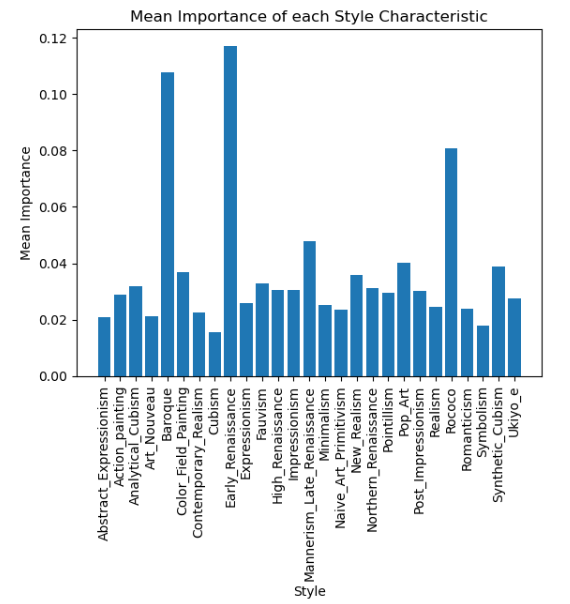
\includegraphics[width=0.70\linewidth]{images/mean_importance.png}
    \caption{Mean importance of style characteristics across 20 classifiers}
    \label{F:1}
\end{figure}


\begin{table}[]
\centering
\begin{tabular}{|l|l|}
\hline
\multicolumn{1}{|c|}{Deep Feature} & MCC \\ \hline
1064 & 0.46 \\ \hline
1106 & 0.22 \\ \hline
1185 & 0.23 \\ \hline
1189 & 0.20 \\ \hline
1302 & 0.18 \\ \hline
1462 & 0.13 \\ \hline
1501 & 0.22 \\ \hline
1643 & 0.38 \\ \hline
1886 & 0.19 \\ \hline
2018 & 0.33 \\ \hline
279 & 0.31 \\ \hline
388 & 0.31 \\ \hline
564 & 0.45 \\ \hline
617 & 0.29 \\ \hline
624 & 0.28 \\ \hline
666 & 0.18 \\ \hline
667 & 0.22 \\ \hline
758 & 0.25 \\ \hline
942 & 0.33 \\ \hline
945 & 0.18 \\ \hline
\end{tabular}
\caption{MCC performance for GBC to classify dominant deep features}
\label{tab:my-table}
\end{table}

\begin{figure}[]
    \centering
    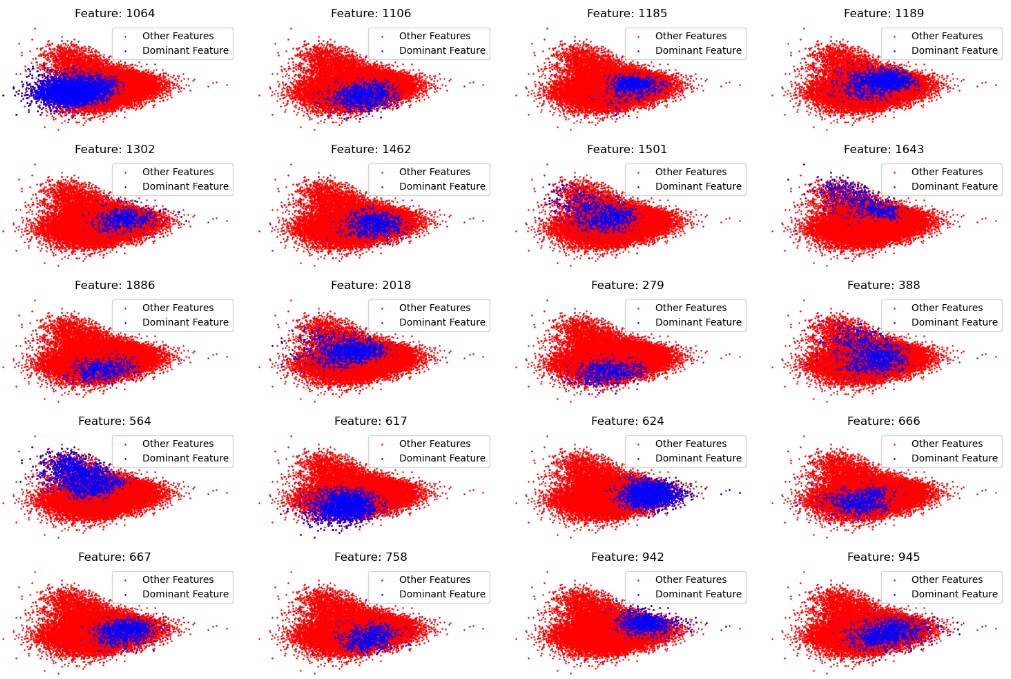
\includegraphics{images/PCA_deep_features.png}
    \caption{PCA projection for each deep feature}
    \label{F:1}
\end{figure}




\end{document}
